\documentclass[]{article}
\usepackage{caption,subcaption,graphicx,float,url,amsmath,amssymb,tocloft}
\usepackage[hidelinks]{hyperref}
\usepackage[toc,acronym,nonumberlist]{glossaries}
\setacronymstyle{long-short}
\usepackage{glossaries-extra}
\graphicspath{{figs/}}
\setlength{\cftsubsecindent}{0em}
\setlength{\cftsecnumwidth}{3em}
\setlength{\cftsubsecnumwidth}{3em} 
%opening
\title{Notes from Origins of Life\\Week4: Early Life}
\author{Simon Crase}

\makeglossaries

\loadglsentries{glossary-entries}

\renewcommand{\thesection}{4.\arabic{section}}
\renewcommand{\glstextformat}[1]{\textbf{\em #1}}

\begin{document}

\maketitle

\begin{abstract}
   These are my notes from the $4^{th}$ week of the Santa Fe Institute Origins of Life Course\cite{sfi2019}. The course aims to push the field of Origins of Life research forward by bringing new and synthetic thinking to the question of how life emerged from an abiotic world.\\
   The content and images contained herein are the intellectual property of the Santa Fe Institute, with the exception of any errors in transcription, which are my own.
   These notes are distributed in the hope that they will be useful,
   but without any warranty, and without even the implied warranty of
   merchantability or fitness for a particular purpose. All feedback is welcome,
   but I don't necessarily undertake to do anything with it.
\end{abstract}

\setcounter{tocdepth}{2}
\tableofcontents
\listoffigures
\section{Introduction}

Lecturer: Chris Kempes


We'll discuss evolution in a pre-cellular world, chemical signatures of early life, protocells, and what the \gls{gls:LUCA} might have looked like.

\section{Protocells}

Lecturer: Sarah Mauer

We'll look at Protocells as a model for the origins of life. Aggregates are important for the origins of life--Figure \ref{fig:ImportanceOfAggregation}.

\begin{itemize}
	\item  Co-localize metabolic/genetic components
	\item   Define the individual to allow for 	selection
	\item   Direct involvement in metabolism
	\begin{itemize}
		\item 	Chemical gradients
		\item   Electron transfer reactions
		\item   Catalytic
	\end{itemize}
	\item   Protect metabolic/genetic 	components
\end{itemize}

\begin{figure}[H]
	\caption{Importance of aggregates to origins of life}\label{fig:ImportanceOfAggregation}
	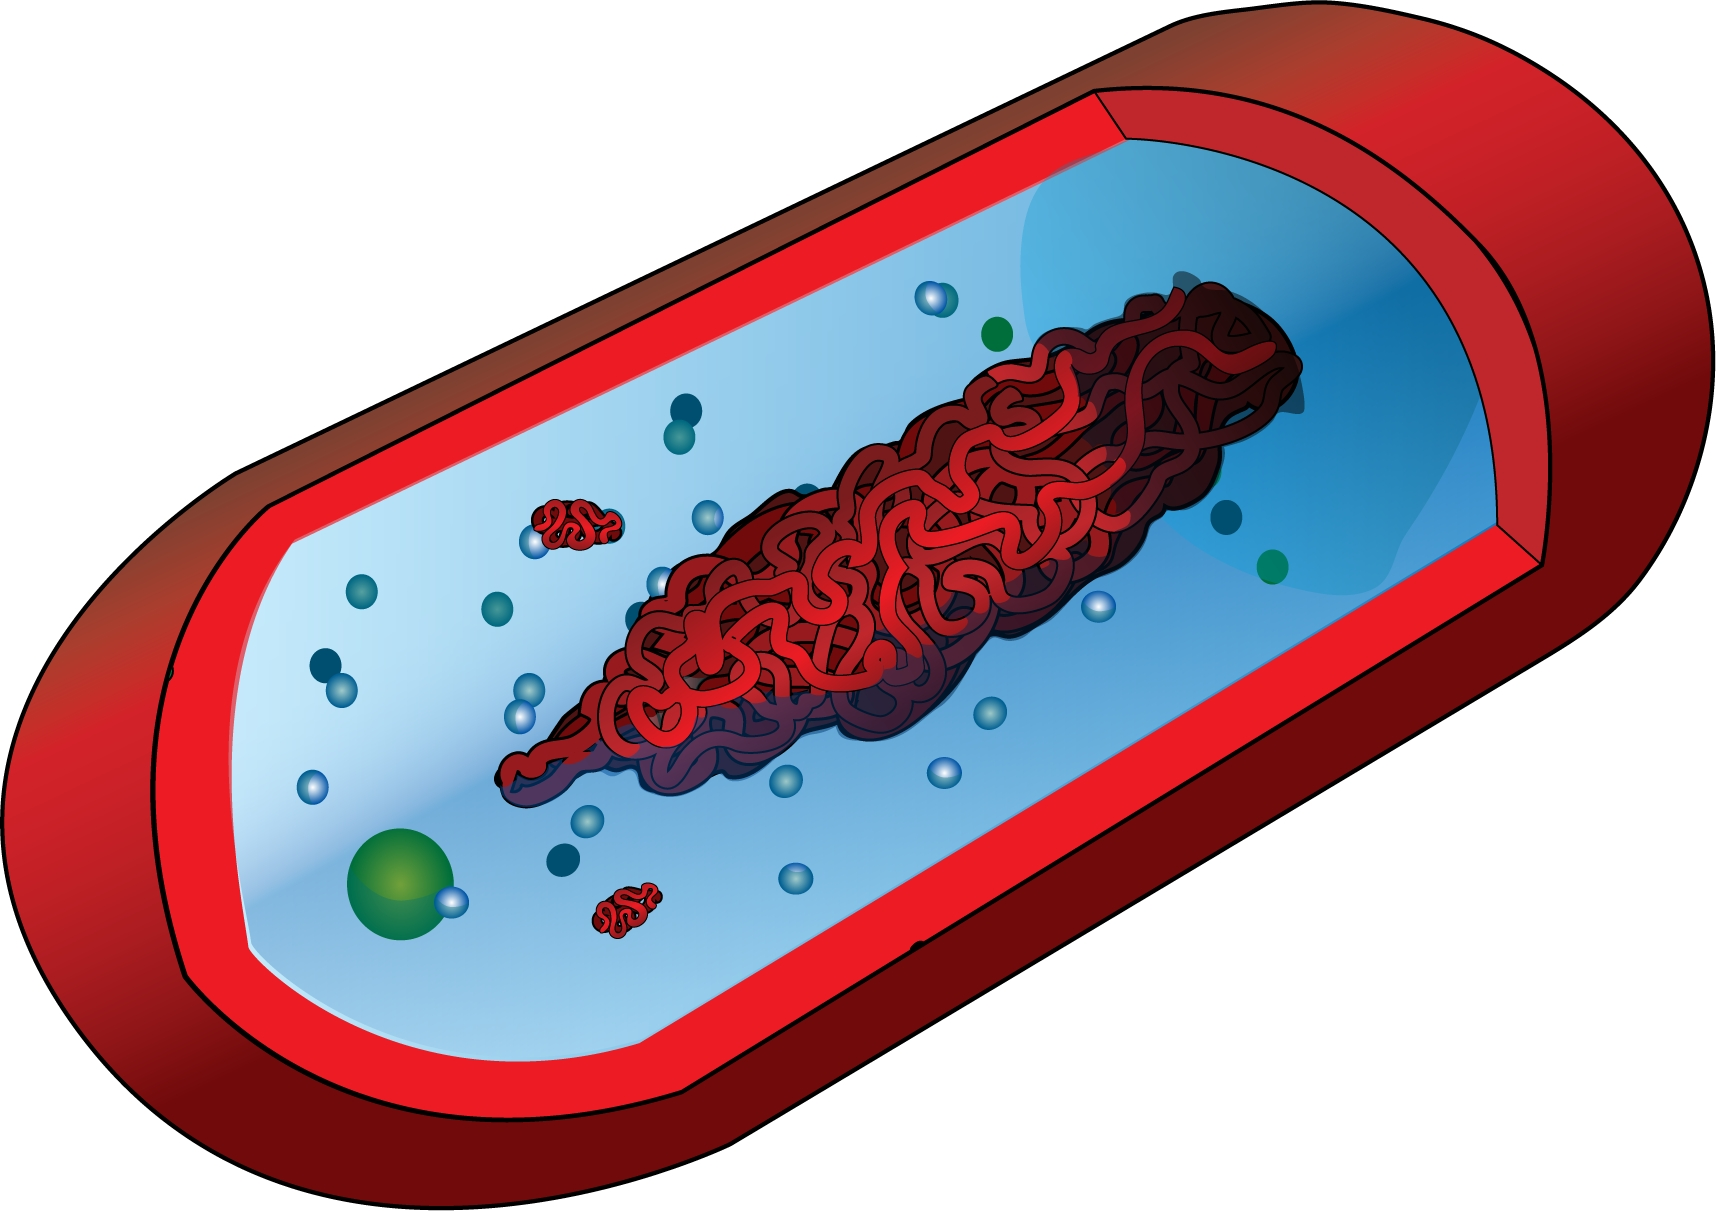
\includegraphics[width=0.9\textwidth]{ImportanceOfAggregation}
\end{figure}

See  \cite{deamer2017role},\cite{maurer2011primitive}, \cite{segre2001lipid}

Self-assembled structures

Controlled by the hydrophobic effect (entropy) and non-bonding interactions (e.g., hydrogen bonds)

\begin{table}[H]
	\caption{Aggregates that are used to model the origins of life}
	\begin{tabular}{l|p{4cm}|p{3cm}} \hline
		Type & Definition &Biological example\\ \hline
		Vesicle (Liposome)& Bilayer-enclosed aqueous compartment& Cells, membrane bound organelles,\\ \hline
		Oil droplet&
		Nonpolar bulk phase often stabilized by
		amphiphiles&
		Lipoproteins (LDL)\\ \hline
		Coacervate&
		\glsdesc{gls:coacervate}&
		P-bodies, membrane-less organelles\\ \hline
		Inorganic&&Thin films or crystals\\ \hline
	\end{tabular}
\end{table}


\begin{figure}[H]
	\centering
	\caption{Self-assembled structures}
	\label{fig:self-assembled-structures}
	\begin{subfigure}[b]{0.3\textwidth}
		\centering
		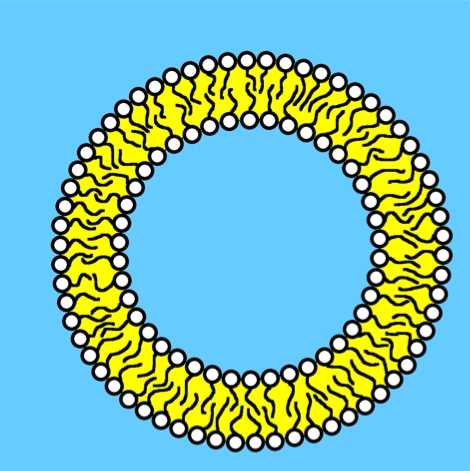
\includegraphics[width=\textwidth]{SelfAssembled1}
		\caption{Water}
		\label{fig:water}
	\end{subfigure}
	\hfill
	\begin{subfigure}[b]{0.3\textwidth}
		\centering
		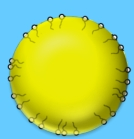
\includegraphics[width=\textwidth]{SelfAssembled2}
		\caption{Not water}
		\label{fig:not-water}
	\end{subfigure}
	\hfill
	\begin{subfigure}[b]{0.3\textwidth}
		\centering
		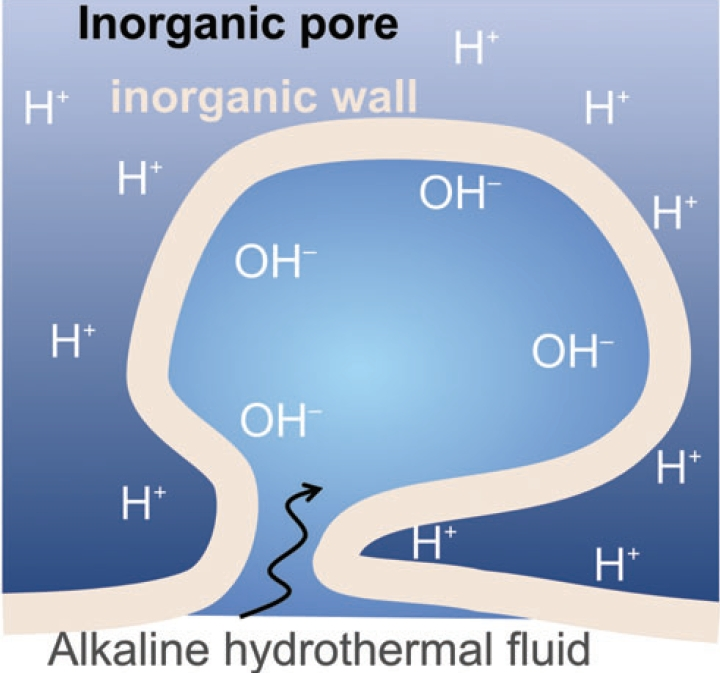
\includegraphics[width=\textwidth]{SelfAssembled3}
		\caption{Proton Gradient across thin inorganic barrier}
		\label{fig:proton-gradient}
	\end{subfigure}

\end{figure}

See \cite{sojo2016origin}

Factors that affect aggregation:
\begin{itemize}
	\item concentration;
	\item temperature;
	\item ionic strength;
	\item pH.
\end{itemize}

What chemistries do protocells harbour? Figure \ref{fig:ProtocellsAndReactions1} shows several possibilities:
\begin{itemize}
	\item A molecules interact with surface of aggregate through electrostatic interactions or hydrogen bonding;
	\item B hydrophobic effect sequestering non-polar molecule;
	\item C amphiphillic molecule anchored in membrane; 
	\item D molecule sequestered but still in water phase.
\end{itemize}

\begin{figure}[H]
	\caption{Aggregates interacting with molecules that are going to start life}\label{fig:ProtocellsAndReactions1}
	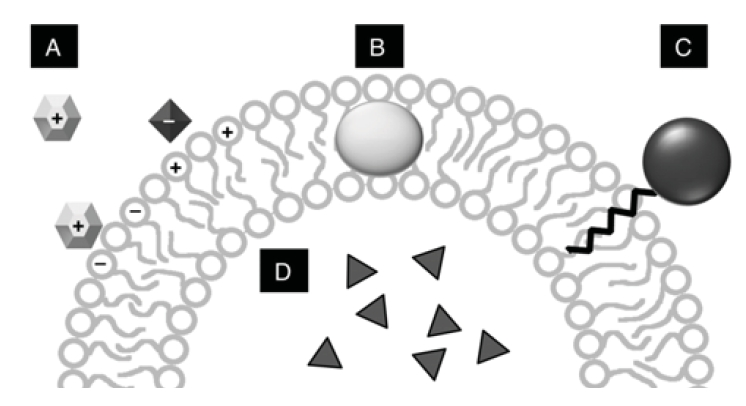
\includegraphics[width=0.9\textwidth]{ProtocellsAndReactions1}
\end{figure}

Figure \ref{fig:ProtocellsAndReactions2} depicts two locations for reactions.
\begin{itemize}
	\item A Surface associated reaction. Substrate becomes Product + Waste, and Waster drifts away. 
	\item B Catalytic network inside membrane, so we need to get rid of Waste.
\end{itemize}
\begin{figure}[H]
	\caption{Two locations for reactions}\label{fig:ProtocellsAndReactions2}
	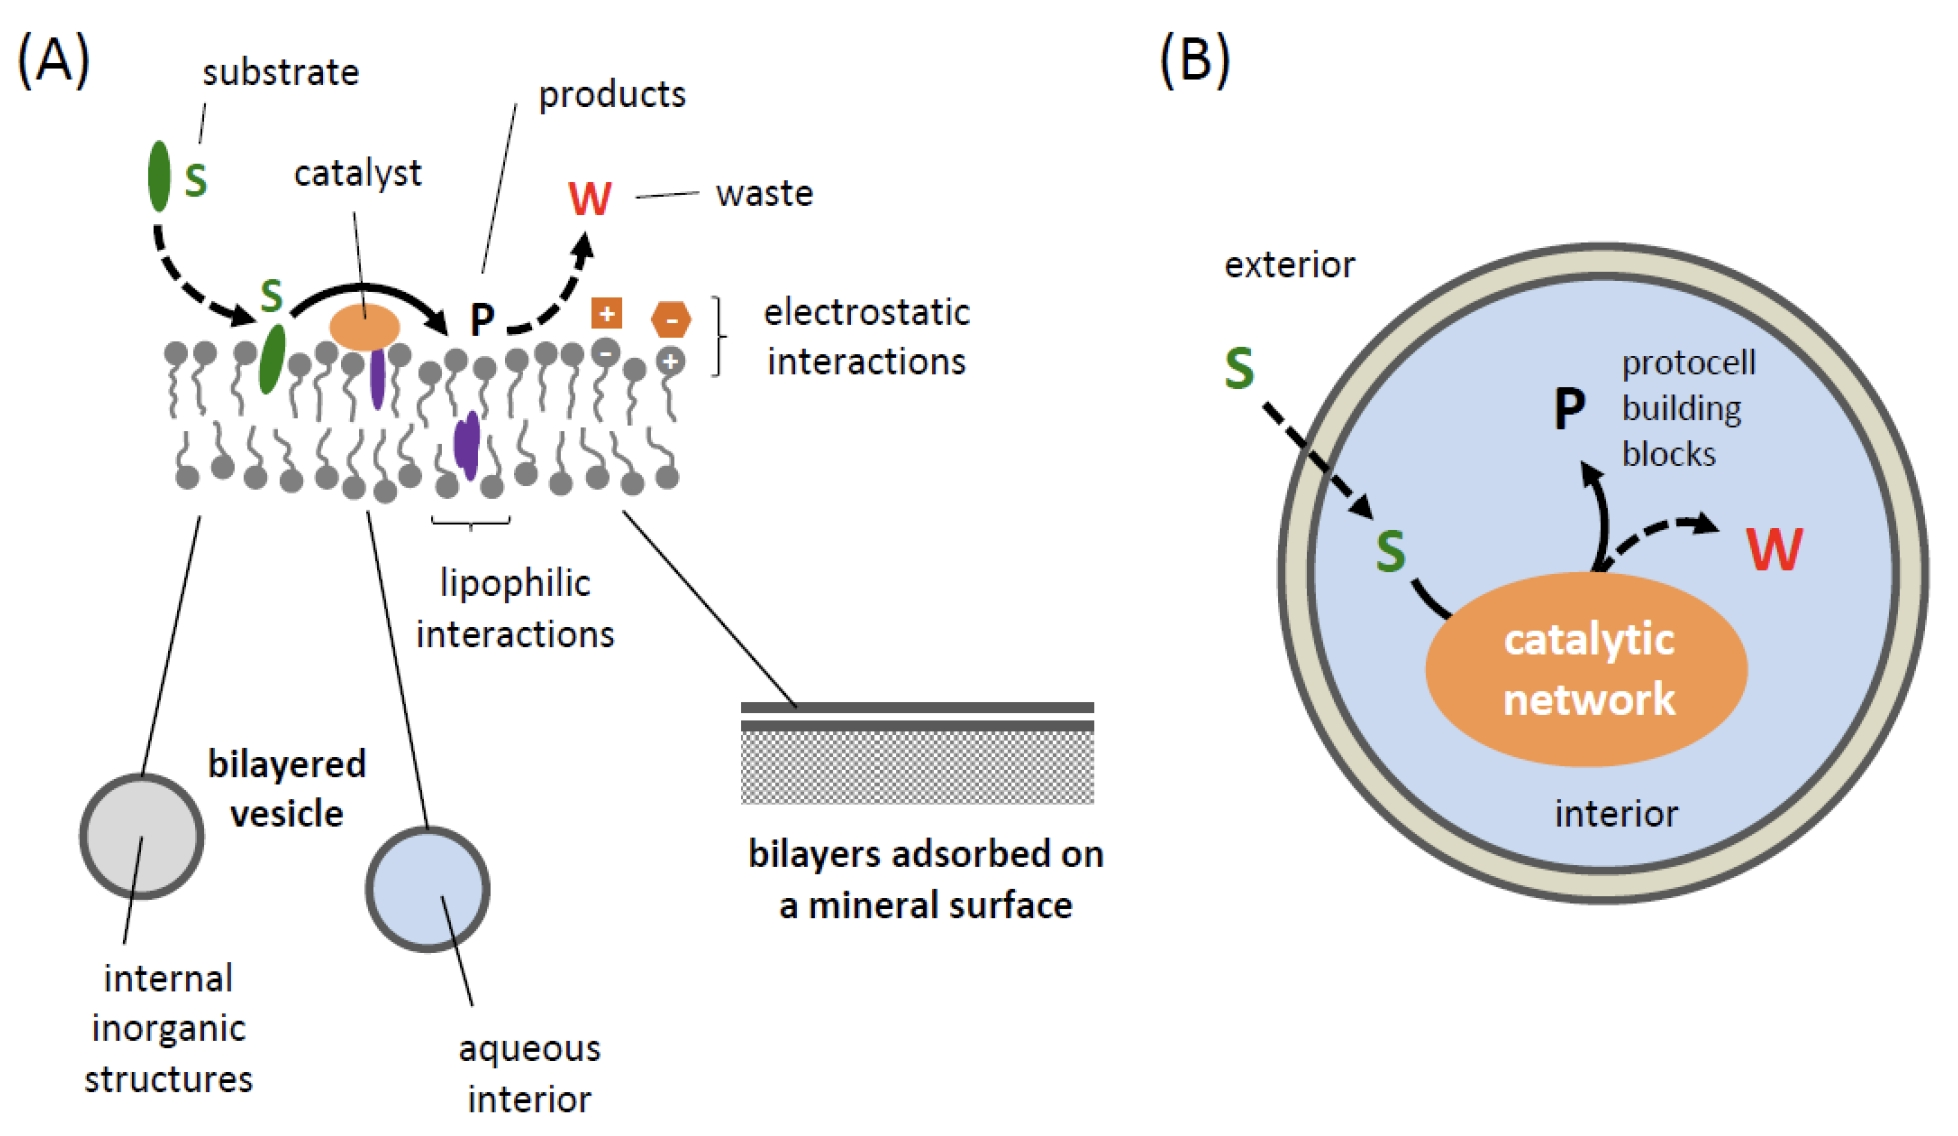
\includegraphics[width=0.9\textwidth]{ProtocellsAndReactions2}
\end{figure}

Figure \ref{fig:ProtocellsAndReactions3} shows an example of a reaction:  the Hammerhead ribosome can self cleave at the red arrow. On the right we see that the reaction is not as fast when it is enclosed in a vesicle, because the waste products can't drain away.


\begin{figure}[H]
	\caption{Example of reaction: the Hammerhead ribosome}\label{fig:ProtocellsAndReactions3}
	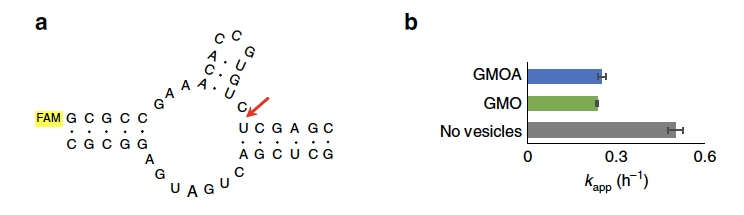
\includegraphics[width=0.9\textwidth]{ProtocellsAndReactions3}
\end{figure}



See \cite{adamala2016programmable} and \cite{monnard2015current}.

See movie, where we see growing vesicle stealing material from neighbour. 
Figure \ref{fig:ProtocellGrowthDivision} illustrates Protocell Growth and division.  

\begin{figure}[H]
	\caption{Protocell Growth and division}\label{fig:ProtocellGrowthDivision}
	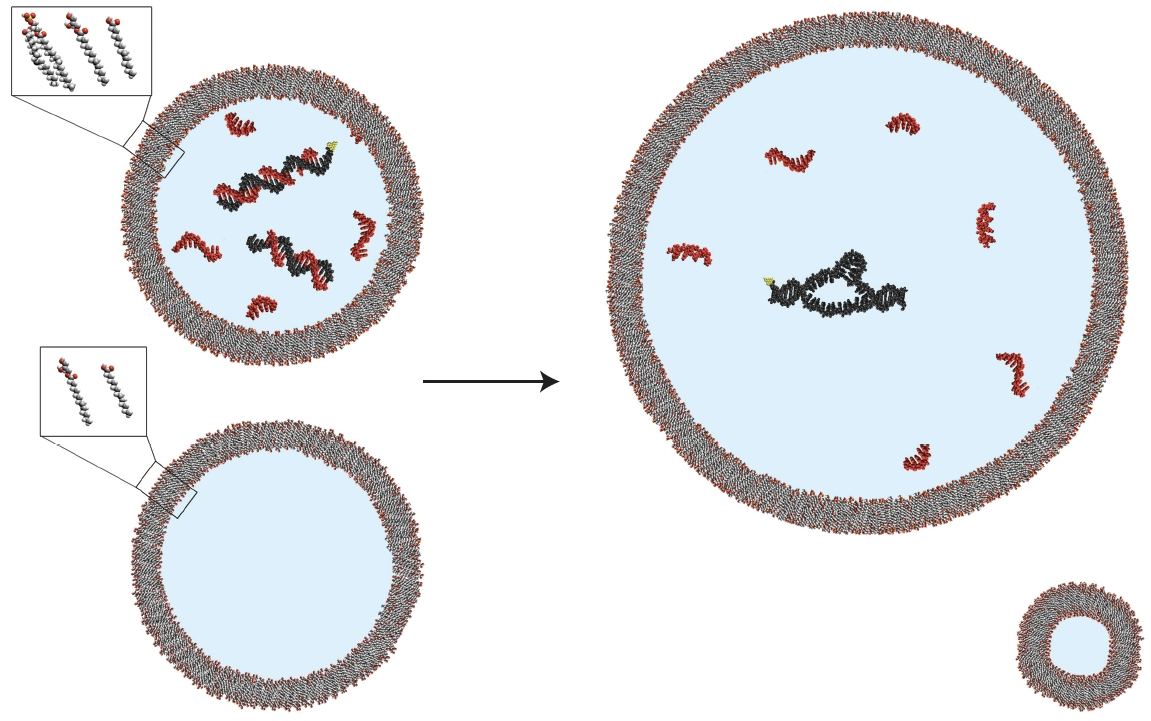
\includegraphics[width=0.9\textwidth]{ProtocellGrowthDivision}
\end{figure}

See  \cite{zhu2012photochemically} and   \cite{chen2004emergence}.

In Figure \ref{fig:TowardsLUCA} we see a prebiotic soup, aggregating, decreasing molecular diversity and increasing functional complexity, and moving towards first life. First life can undergo Darwinian evolution towards \gls{gls:LUCA}.
\begin{figure}[H]
	\caption{Towards LUCA}\label{fig:TowardsLUCA}
	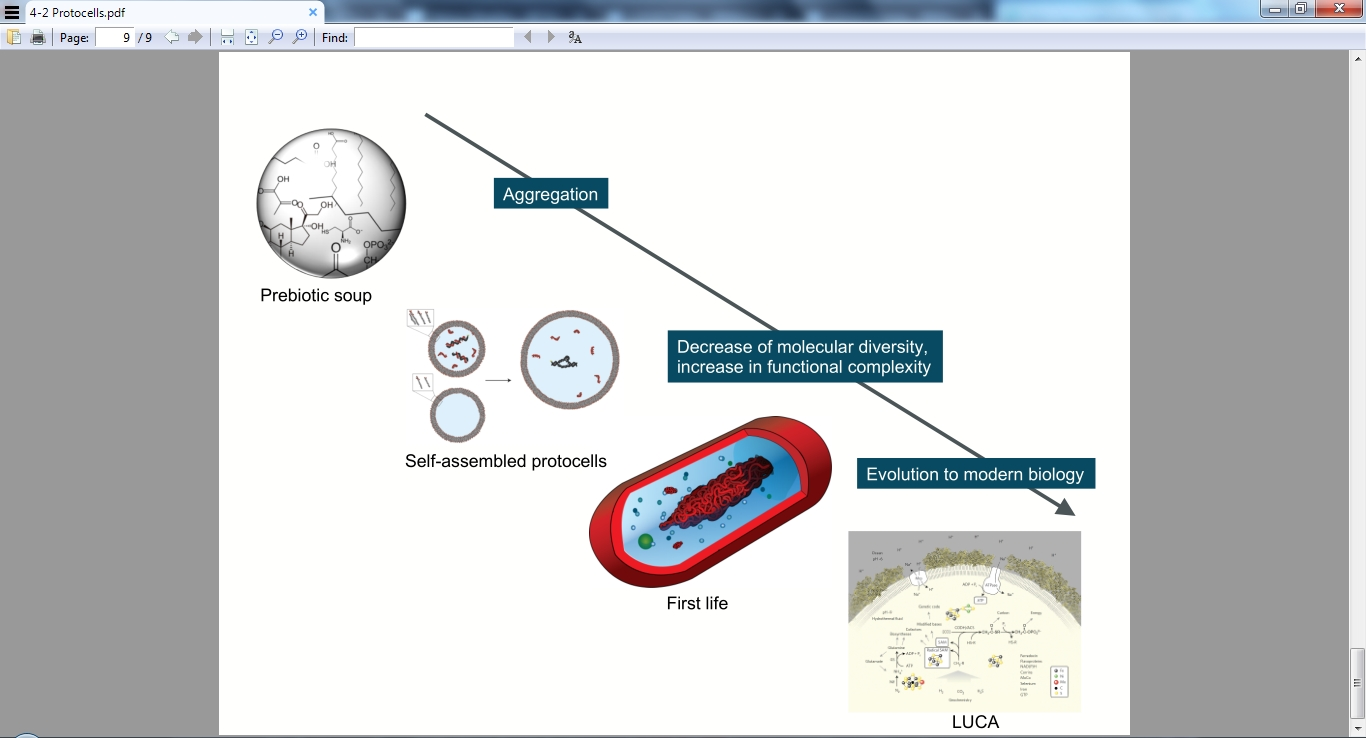
\includegraphics[width=0.9\textwidth]{TowardsLUCA}
\end{figure}

\section{LUCA}

Lecturer: Kate Adamala

Kate discusses the Last Universal Common Ancestor of all Life.

The modern Tree of Life--Figure \ref{fig:TOL4}\cite{hug2016new}-- is very diverse in physiology, morphology, and life strategies. But all the diversity  comes from one single ancestor--Figure \ref{fig:TOL_root}.
\begin{figure}[H]
	\caption{The modern Tree of Life}\label{fig:TOL4}
	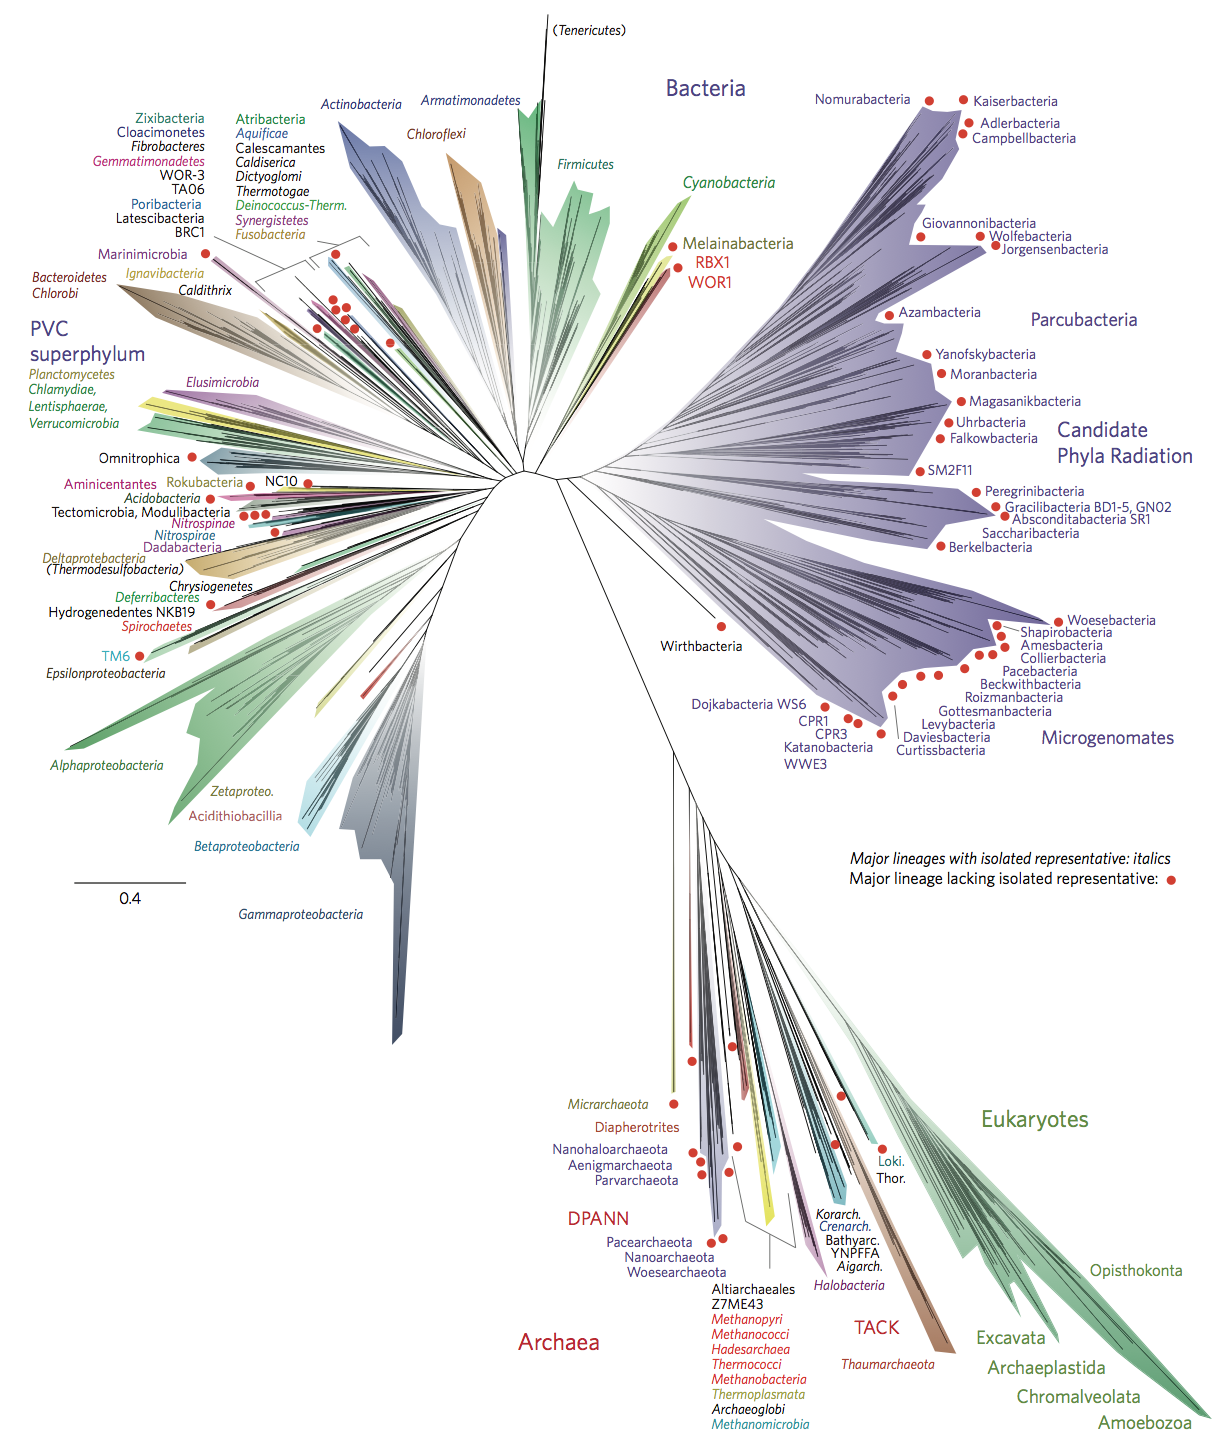
\includegraphics[width=\textwidth]{A_Novel_Representation_Of_The_Tree_Of_Life}
\end{figure}

\begin{figure}[H]
	\caption{All the diversity of Figure \ref{fig:TOL4} comes from one single ancestor.}\label{fig:TOL_root}
	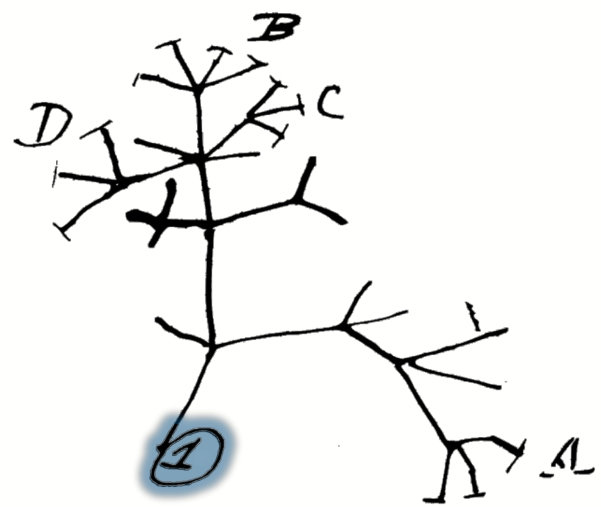
\includegraphics[width=0.9\textwidth]{TOL_root}
\end{figure}

We know that all life came from one population of earliest cells; we know this because all modern life is built on the same principles--Figure \ref{fig:ModernCell}. At one stage, all of life went through the stage of a very simple cell, \gls{gls:LUCA}--Figure \ref{fig:EvolCell}.

\begin{figure}[H]
	\caption{All life came from one population of earliest cells}\label{fig:ModernCell}
	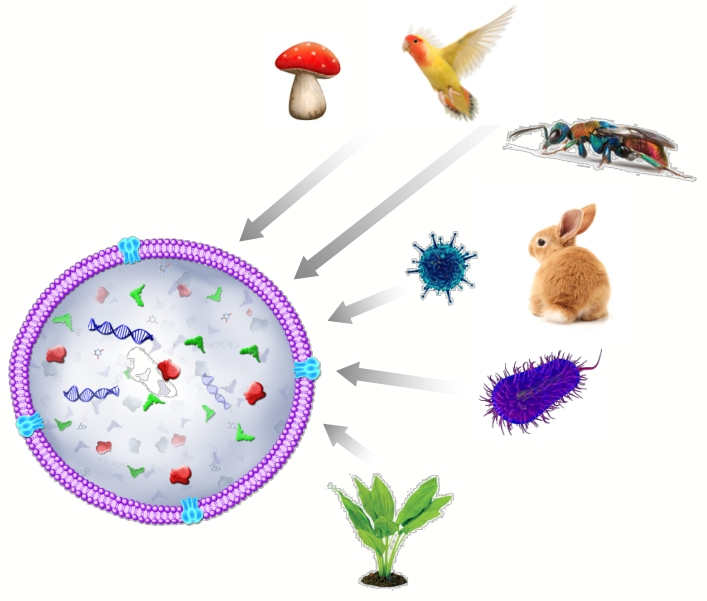
\includegraphics[width=0.9\textwidth]{ModernCell}
\end{figure}

\begin{figure}[H]
	\caption{Evolution of Life, showing very simple cell, LUCA}\label{fig:EvolCell}
	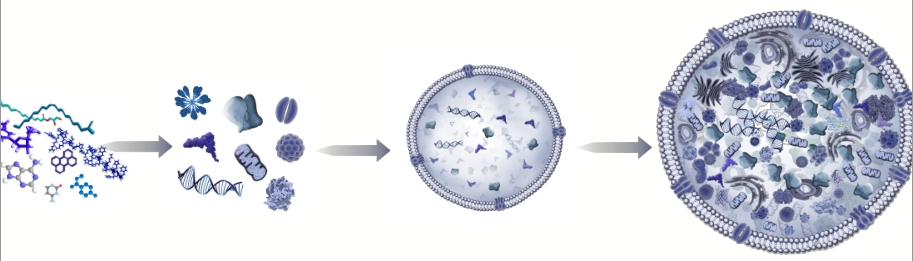
\includegraphics[width=0.9\textwidth]{EvolCell}
\end{figure}

\gls{gls:LUCA} was the ancestor to all modern cells, so it must have possessed the basic mechanisms of  modern cells.

\begin{figure}[H]
	\caption{LUCA must have possessed the basic mechanisms of  modern cells}\label{fig:LUCA_Attributes}
	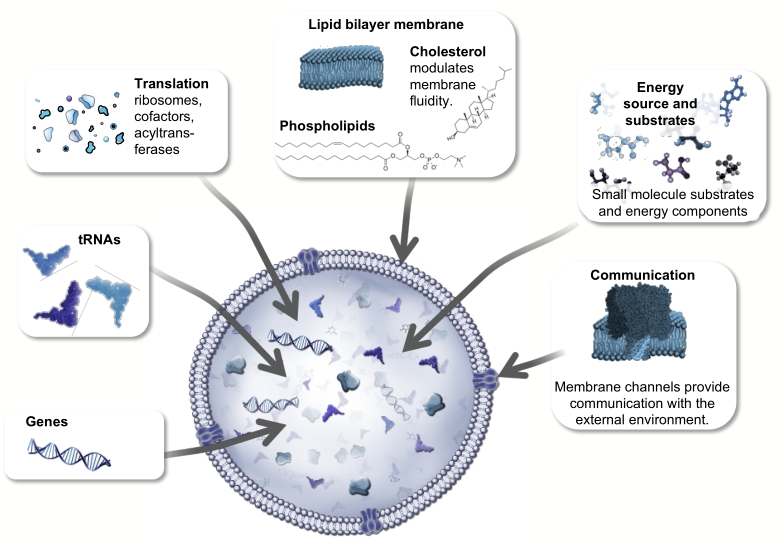
\includegraphics[width=0.9\textwidth]{LUCA_Attributes}
\end{figure}

We know quite a lot about LUCA, but much is still unknown. We can deduce much by studying biochemical evolution and thr properties of modern cells to see what they share.

References:
\begin{itemize}
	\item \cite{penny1999nature}--cytology of PUCA;
	\item \cite{weiss2016physiology}--phylogenomic analysis to determine genome of LUCA;
	\item \cite{torino2013piecing}--reconstruct LUCA in ther lab.
\end{itemize}

\section{Chemical signatures for identifying life in the geological record}

Lecturer: Mayuko Nakagawa

Contents
\begin{itemize}
	\item About Biogeochemistry
	\item Fingerprints of life and environment
	\begin{itemize}
		\item Fossils
		\item Mineral compositions
		\item Isotopic signatures
	\end{itemize}
	\item How to use the signatures for identifying lives from 	Earth geological records?
\end{itemize}

Biogeochemistry--The study of:
\begin{itemize}
	\item How chemical elements flow through living systems and their physical environments--Figure \ref{fig:Biogeochemistry}\cite{linares-pasten_2018}.
	\item Investigate the factors that influence cycles of key 	elements such as bioelements (C, H, N, O, S...).
	
\end{itemize}

\begin{figure}[H]
	\caption{How chemical elements flow through living systems}\label{fig:Biogeochemistry}
	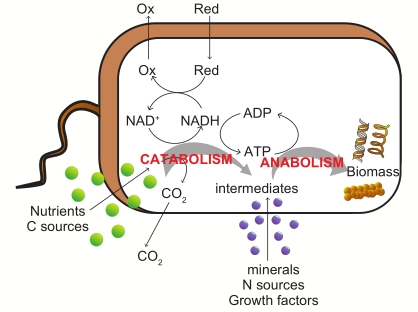
\includegraphics[width=0.9\textwidth]{Biogeochemistry}
\end{figure}

Fingerprints of Life
\begin{itemize}
	\item  DNA information cannot be preserved over geologic time
	scale (thousands ~ million years for eukaryotes' DNA)
	\item Chemical and morphological signatures are utilized
	\begin{itemize}
		\item  Fossils, molecular fossils
		\item Mineral compositions
		\item Isotopic signatures
	\end{itemize}
\end{itemize}

Isotopic signatures: Isotope variants of a particular chemical element
which differ in neutron number
\begin{itemize}
	\item  Stable isotope
	\begin{itemize}
		\item do not decay into other
		elements.
		\item Behavior is slightly different by the
		mass, useful for understanding
		material cycle.
	\end{itemize}
	\item Radioactive isotope: one having an unstable nucleus and
	which emits characteristic radiation during
	its decay to a stable form- e.g. $^3H$, $^14C$
\end{itemize}

\begin{figure}[H]
	\caption{Carbon Isotopes}\label{fig:CarbonIsotopes}
	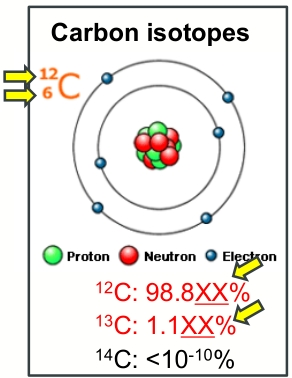
\includegraphics[width=0.9\textwidth]{CarbonIsotopes}
\end{figure}

Isotopic Signatures

\begin{itemize}
	\item \textit{Kinetic isotopic effect}:
	Isotope ratio is changed by kinetic reactions 	(e.g.) the isotopic ratios are changed between substrates and products reflecting the metabolic processes. \begin{align*}
	^{12}CO_2 + H_2O \rightarrow&^{12}CH_2O + O_2 \text{, runs slightly faster than}\\
	^{13}CO_2 + H_2O \rightarrow&^{13}CH_2O + O_2 
	\end{align*}
	\item \textit{Equilibrium isotopic effect}:
	Isotope ratio is changed by equilibrium reactions.
	e.g.) Temperature effect, phase (gas, liquid, solid)
	$^{18}O$ ( $^{16}O$) is more (less) enriched in liquid than gas phase
\end{itemize}

\begin{figure}[H]
	\caption{Earth environment interacts with origin and evolution of life}\label{fig:Timeline}
	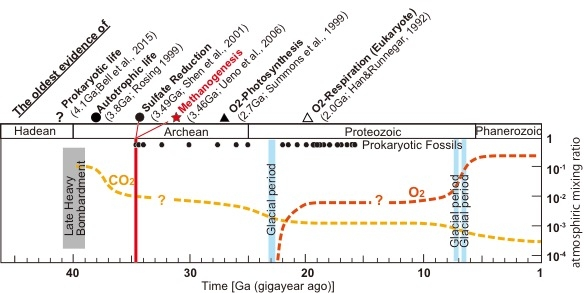
\includegraphics[width=0.9\textwidth]{Timeline}
\end{figure}

\begin{itemize}
	\item O2 level is important for evolution of life:
	\begin{itemize}
		\item the content of oxidized minerals and S isotope ratios are used for
		signatures of O2 level
	\end{itemize}
	\item  Small C isotope ratio ($\delta^{13}C$) of microfossils
	\begin{itemize}
		\item 	The difference of $\delta^{13}C$ values between carbonate and organic carbon ($<13\%$) indicated the possibility of Acetyl-CoA pathway
		and/or Calvin cycle product.
	\end{itemize}
\end{itemize}

Isotopic signature for Methanogens:
\begin{itemize}
	\item The sample rocks ($\approx 3.5Ga$); at the Dresser Formation at the North Pole area in Pilbara craton, Western Australia \cite{ueno2006evidence},
	\item Fluid inclusion; Tiny bubble of liquid or gas trapped inside a solid mineral-phase--Figure \ref{fig:FluidInclusionInTheRock}
	\item Measure C isotope ratio ( $\delta^{13}C$) of $CO_2$ and $CH_4$ in fluid inclusion
\end{itemize}

\begin{figure}[H]
	\caption{Fluid inclusion in the rock}\label{fig:FluidInclusionInTheRock}
	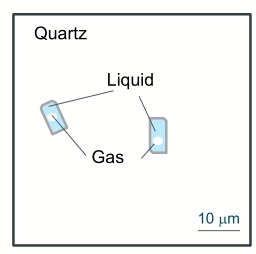
\includegraphics[width=0.9\textwidth]{FluidInclusionInTheRock}
\end{figure}

Isotopic signature for Methanogens. Figure \ref{fig:ueno_comparison} supports the idea that the methane is biogenic.
\begin{itemize}
	\item Methane production processes (Biogenic)
	\begin{itemize}
		\item 	Acetate Fermentation
		\item $CO_2$ reduction
	\end{itemize}
	\item Methane production processes (Abiotic)
	\begin{itemize}
		\item Thermogenic decomposition,
		\item Fischer-Tropsch reaction
	\end{itemize}
\end{itemize}

\begin{figure}[H]
	\caption{Comparison with present-day hydrothermal system}\label{fig:ueno_comparison}
	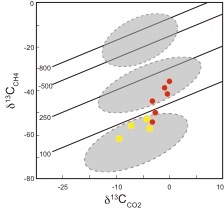
\includegraphics[width=0.9\textwidth]{ueno_comparison}
\end{figure}

Take Home Message: Signatures of life:
\begin{itemize}
	\item Chemical signatures, especially stable isotope information, are important tool for identifying the biogenic signatures preserved in geological records
	\item To understand how to record and decode the signatures, researches on modern earth material cycle and organisms are 	necessary.
\end{itemize}

Suggested Reading:

\cite{sharp2017principles} and \cite{allegre2008isotope}

References:
\cite{ueno2006evidence},
 \cite{bell2015potentially}, \cite{rosing199913c},  \cite{shen2001isotopic}, \cite{summons19992}, \cite{han1992megascopic}

\section{RNA}

\subsection{The RNA World}

Lecturer: Tony Z. Jia

Figure {fig:ModernCellSchematic} shows the modern cell, with a lipid membrane and processes catalyzed by proteins and ribosomes. These process give rise to the Central Dogma--Figure \ref{fig:CentralDogmaModernCell}.
\begin{figure}[H]
	\caption{The Modern Cell}\label{fig:ModernCellSchematic}
	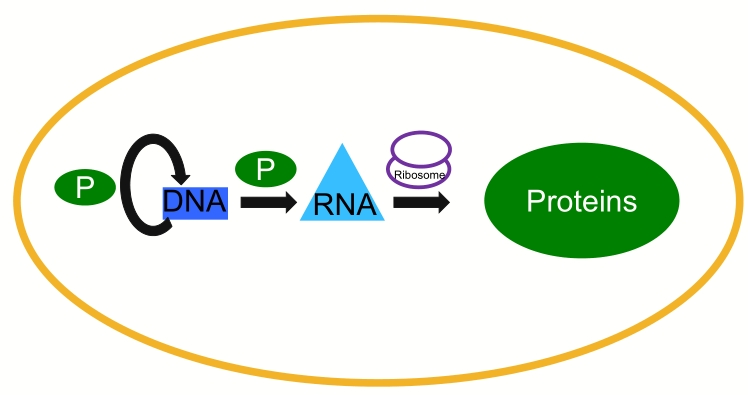
\includegraphics[width=0.9\textwidth]{ModernCellSchematic}
\end{figure}

\begin{figure}[H]
	\caption{The Central Dogma}\label{fig:CentralDogmaModernCell}
	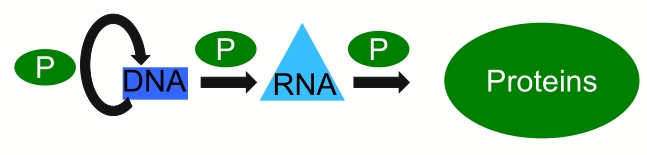
\includegraphics[width=0.9\textwidth]{CentralDogmaModernCell}
\end{figure}

RNA World Theory.
\begin{itemize}
	\item  RNA can store and pass down genetic information--Figure \ref{fig:RNA_WorldTheory}
	\item  RNA can catalyze chemical processes (ribozymes)--Figure \ref{fig:RNA_can_catalyze_chemical_processes}\cite{scott2013hammerhead}
\end{itemize}
\begin{figure}[H]
	\caption{RNA can store and pass down genetic information similar to DNA}\label{fig:RNA_WorldTheory}
	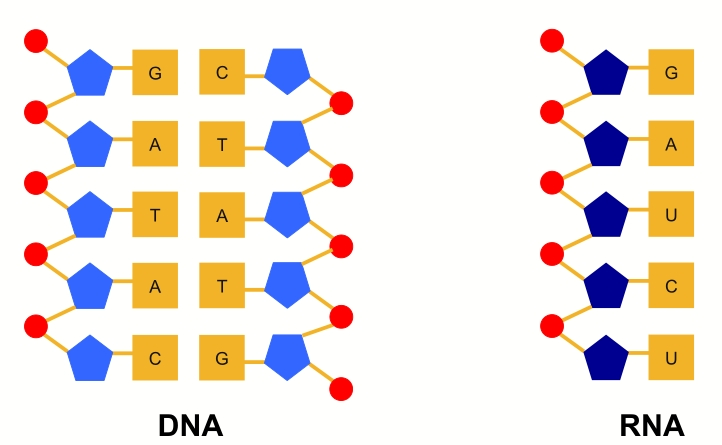
\includegraphics[width=0.9\textwidth]{RNA_WorldTheory}
\end{figure}

\begin{figure}[H]
	\caption{RNA can catalyze chemical processes}\label{fig:RNA_can_catalyze_chemical_processes}
	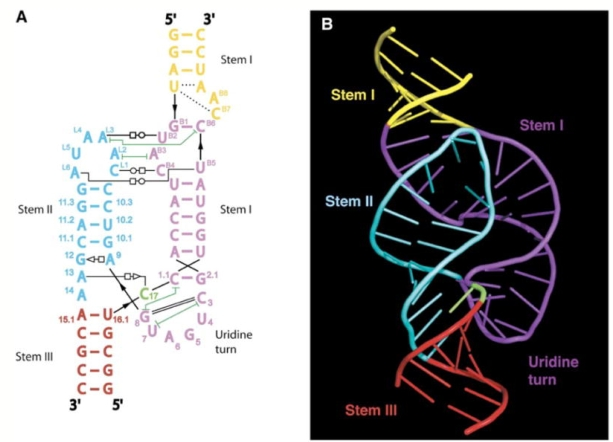
\includegraphics[width=0.9\textwidth]{RNA_can_catalyze_chemical_processes}
\end{figure}

We'll consider an early living system--Figure \ref{fig:RNA_WorldTheory1}\cite{blain2014progress}, where the genetic material is RNA:
\begin{itemize}
	\item need RNA to be able to replicate and evolve;
	\item then system can grow, replicate, and divide.
\end{itemize}
 

\begin{figure}[H]
	\caption{An early living system, where the genetic material is RNA.}\label{fig:RNA_WorldTheory1}
	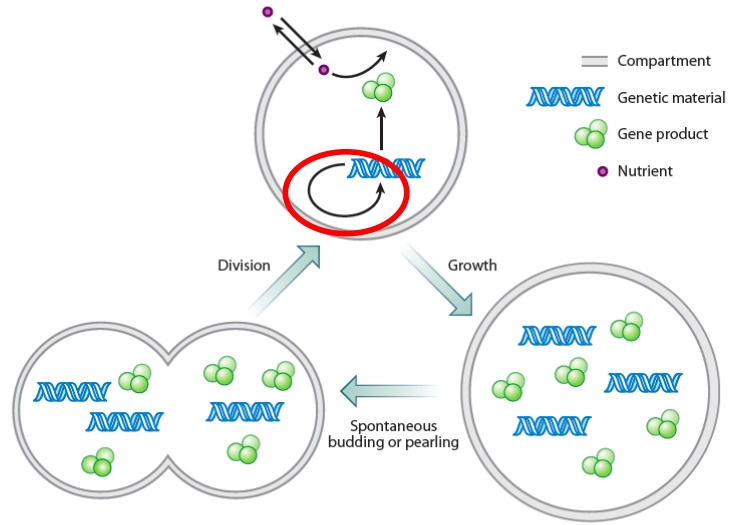
\includegraphics[width=0.9\textwidth]{RNA_WorldTheory1}
\end{figure}

There are many ways this has been postulated to occur. At some point in evolution. It is likely that an RNA ribozyme, i.e. a catalytic RNA that could catalyze replication and polymerization of other RNA molecules, would have been required. But what would have happened before the emergence of such an RNA ribozyme? Figure \ref{fig:NonenzymaticRNA_Polymerization}\cite{blain2014progress} shows one possibility:
\begin{itemize}
	\item monomers bind to RNA, based on complements;
	\item monomers are then polymerized, so we get complementary strand;
	\begin{itemize}
		\item one mechanism involves the Leaving Group\footnote{All Leaving Groups discussed here are laboratory analogs. They aren't necessarily what was used, but they enable us to study processes in the lab.} in the Template, a slightly activated group that catalyzes extension;
		\item Leaving Group may be 2-Methylimidazole
	\end{itemize} 
	\item at this point, RNA strand has replicated itself.
\end{itemize}


\begin{figure}[H]
	\caption{Nonenzymatic RNA Polymerization}\label{fig:NonenzymaticRNA_Polymerization}
	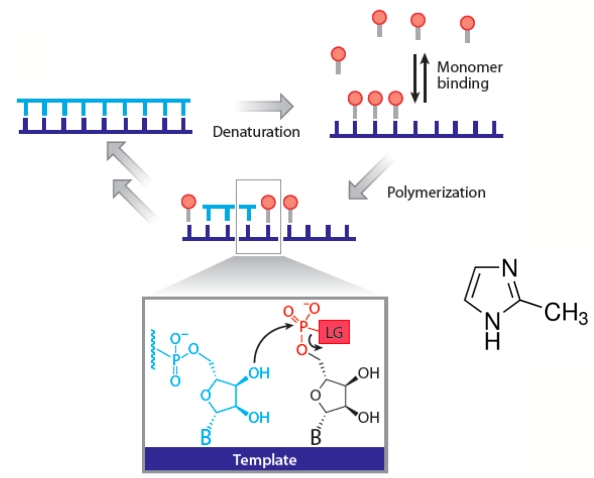
\includegraphics[width=0.9\textwidth]{NonenzymaticRNA_Polymerization}
\end{figure}

There are some outstanding issues:
\begin{itemize}
	\item How does denaturation step happen in Figure \ref{fig:NonenzymaticRNA_Polymerization}? Otherwise we'd use up all RNA, and there would be no evolution. Figure \ref{fig:PrebioticRNA_StrandSeparation} shows one possibility--pH cycling.
	\item Polymerization isn't as fast as we'd like, and there is some degrading. Figure \ref{fig:ChangeLeavingGroup} shows one possibility: replace 2-Methylimidazole with 2-aminoimidazole\cite{li2017enhanced}, which gives a much faster reaction.
	\item  RNA is very labile to hydrolysis, and it \textit{degrades quickly}, especially if solutions aren't clean. Need Magnesium cations for ploymerization, but this also causes degradation. Maybe use a different cation, such as Iron--Figure \ref{fig:RNA_polymerization_via_iron}\cite{blain2014progress}.
\end{itemize}

\begin{figure}[H]
	\caption{Nonenzymatic RNA Polymerization}\label{fig:PrebioticRNA_StrandSeparation}
	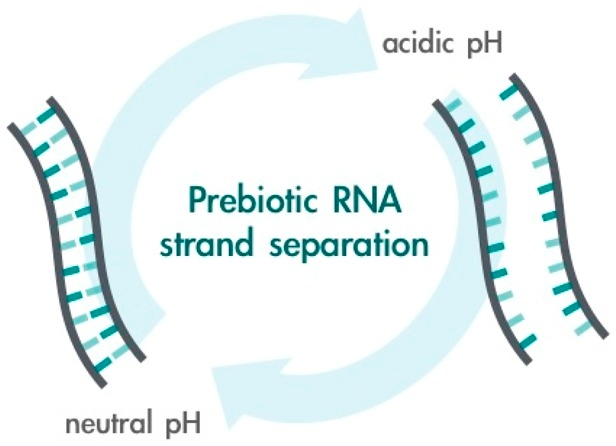
\includegraphics[width=0.9\textwidth]{PrebioticRNA_StrandSeparation}
\end{figure}

\begin{figure}[H]
	\caption{Replace 2-Methylimidazole with 2-aminoimidazole}\label{fig:ChangeLeavingGroup}
	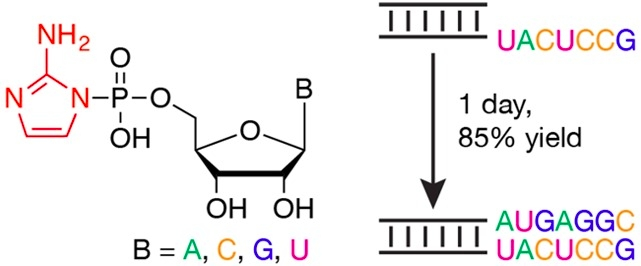
\includegraphics[width=0.9\textwidth]{ChangeLeavingGroup}
\end{figure}

\begin{figure}[H]
	\caption{Use Reduced Iron in an oxygen free chamber.}\label{fig:RNA_polymerization_via_iron}
	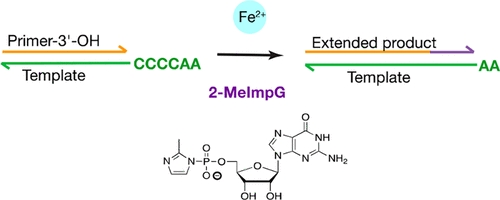
\includegraphics[width=0.9\textwidth]{RNA_polymerization_via_iron}
\end{figure}

See \cite{robertson2012origins} and  \cite{joyce2018protocells} for details of the origins of the RNA world, and its processes, and \cite{hud2018searching} for information on the hypothetical pre-RNA world. Finally, it is possible to have living systems with more than 4 bases  \cite{hoshika2019hachimoji}.

\subsection{Molecular Evolution in the Lab}

Lecturer: Mark A. Ditzler

A method called In vitro evolution allows us to observe the evolution of molecules in a test tube. It has been used to study several classes of molecules:
\begin{itemize}
	\item Proteins
	\item Ribonucleic acids (RNAs)
	\item Non-biological RNA-like molecules (like RNA, but with different backbone or different base-pairs)
\end{itemize}

In vitro evolution allows us to answer two broad questions:
\begin{itemize}
	\item what \textit{can} these molecules do?
	\item how \textit{can} they evolve?
\end{itemize}
This study is independent of biology and specific evolutionary histories.

How does In vitro evolution work--Figure \ref{fig:InVitroEvolution}?

\begin{itemize}
	\item Start with a diverse population, e.g. $\approx 10^{15}$ 
	unique sequences of protein, RNA, or RNA-like molecules
	\item Isolate molecules that have the desired function
	\begin{itemize}
		\item Carry out chemical reactions:
		Ligation, transfer of functional groups,
		oxidation/reduction, isomerization, etc
		\item Bind other biomolecules:
		Wide variety of metabolites and proteins
	\end{itemize}
	\item Use enzymatic steps to make many copies of isolated molecules
	\item There will be some mutations (mistakes), so we get additional diversity
	\item Repeated selection will produce more copies of ''better'' sequences
	\item Repeat until we end up with ''really good'' sequences--Figure \ref{fig:InVitroEvolutionRepeat}
\end{itemize}

\begin{figure}[H]
	\caption{How does In vitro evolution work? First steps.}\label{fig:InVitroEvolution}
	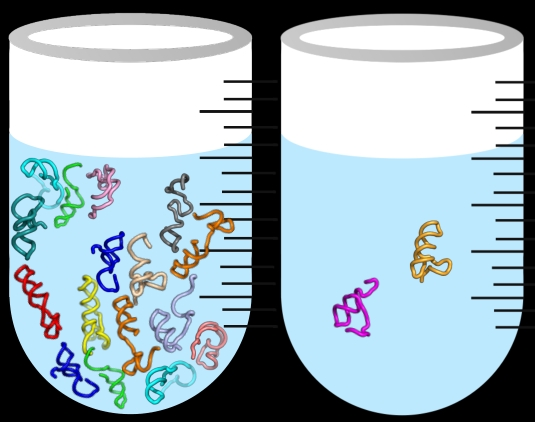
\includegraphics[width=0.9\textwidth]{InVitroEvolution}
\end{figure}

\begin{figure}[H]
	\caption{How does In vitro evolution work? Overview}\label{fig:InVitroEvolutionRepeat}
	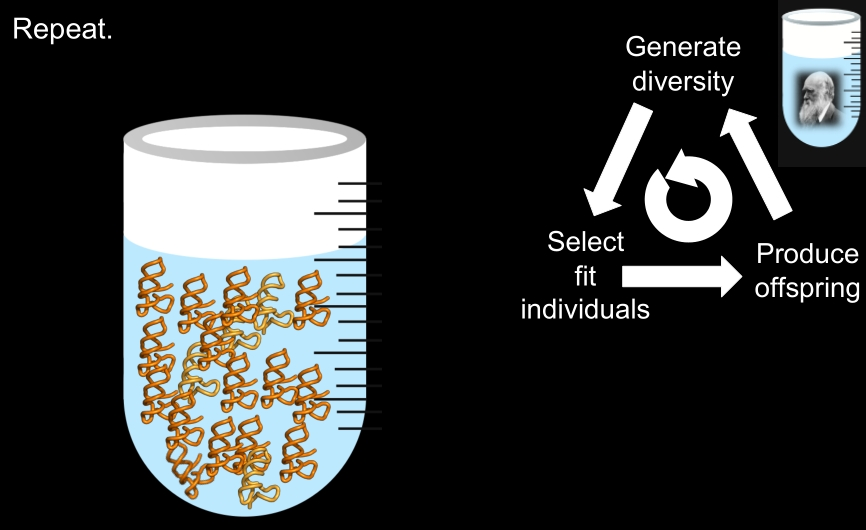
\includegraphics[width=0.9\textwidth]{InVitroEvolutionRepeat}
\end{figure}

What have we learned?
\begin{itemize}
	\item what \textit{can} these molecules do?
	\begin{itemize}
		\item Very simple proteins can carry out chemical reactions\cite{seelig2007selection}
		\item RNA can catalyze many classes of chemical reactions\cite{chen2007ribozyme}
		\item RNA can bind a wide range of biomolecules\cite{gold2012aptamers}
		\item RNA-like molecules can do many of the same functions as RNA\cite{sefah2014vitro} \cite{pinheiro2012synthetic}
	\end{itemize}
	\item how \textit{can} they evolve?
		\begin{itemize}
		\item Proteins evolved in vitro look different from proteins in modern biology\cite{mansy2007structure}
		\item Highly active molecules with complex functions are extremely rare among random sequences \cite{bartel1993isolation}
		\item Neutral point-mutations may plan a smaller role in evolution of new structure and functions than we previously thought\cite{petrie2014limits} \cite{pressman2019mapping}
	\end{itemize}
\end{itemize}

Suggested Reading
\begin{itemize}
	\item \cite{joyce2007forty}This is an excellent review of the history of in vitro evolution as told by one of its most accomplished practitioners.
	\item \cite{seelig2007selection} This paper is an excellent example of the in vitro evolution of a protein
	\item \cite{chen2007ribozyme} This is a very well-written patent filed in 1991 by one of the pioneers of in
	vitro evolution for a specific form of in vitro evolution known as SELEX.
\end{itemize}


\section{Autocatalysis}

\subsection{Autocatalytic Sets: A Cooperative Origin of Life}
\cite{wim2017origin}, \cite{hordijk2017chasing}, \cite{wim2019wandering}, \cite{patzke2007self}, \cite{vaidya2012spontaneous}, \cite{ashkenasy2004design}, \cite{hordijk2012structure}, \cite{sousa2015autocatalytic}

\subsection{Reaction Networks and Autocatalysis}

\section{Evolutionary Theory}

\subsection{An Introduction}

Lecturer: Michael Travisano

Evolutionary origin of three processes--Figure \ref{fig:EvolutionaryOrigin}.

\begin{itemize}
	\item Metabolism
	\item Genetic Transmission
	\item Evolution
\end{itemize}

\begin{figure}[H]
	\caption{Evolutionary origin of three processes}\label{fig:EvolutionaryOrigin}
	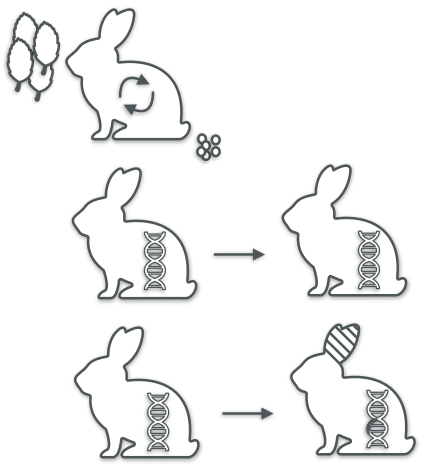
\includegraphics[width=0.9\textwidth]{EvolutionaryOrigin}
\end{figure}

\subsubsection{Metabolism}

Metabolic pathways are complex. It is hard to imagine how we could go from nothing to the Citric Acid Cycle--Figure \ref{fig:CitricAcidCycle}. So metabolism probably started with one of the many non-living metabolism-like processes on Earth, such as the Black Smoker--Figure \ref{fig:BlackSmoker}.
\begin{figure}[H]
	\caption{Metabolic pathways are complex}\label{fig:CitricAcidCycle}
	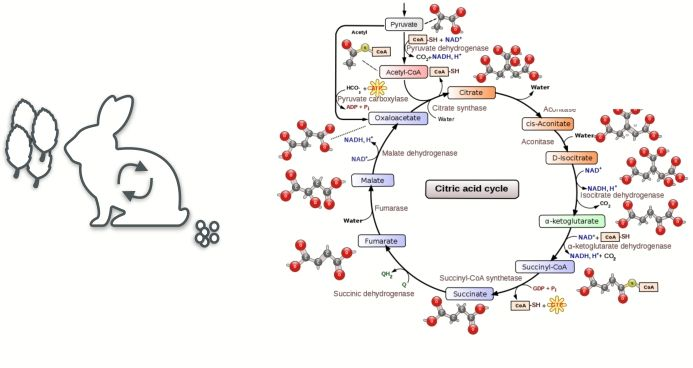
\includegraphics[width=0.9\textwidth]{CitricAcidCycle}
\end{figure}

\begin{figure}[H]
	\caption{Black Smoker: one of the many non-living metabolism-like processes on Earth}\label{fig:BlackSmoker}
	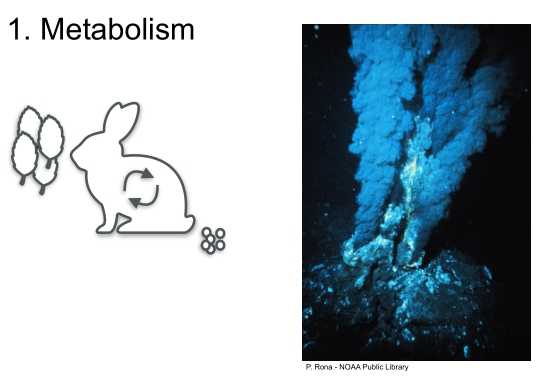
\includegraphics[width=0.9\textwidth]{BlackSmoker}
\end{figure}

\subsubsection{Genetic Transmission}

DNA replication is complex--Figure \ref{fig:DNA_replication_complex}--and this is only one of the processes involved. Figure \ref{fig:SpontaneousFormation}\cite{cafferty2016spontaneous} illustrates some possible precursors which self-assemble in water. 
\begin{figure}[H]
	\caption{DNA replication is complex}\label{fig:DNA_replication_complex}
	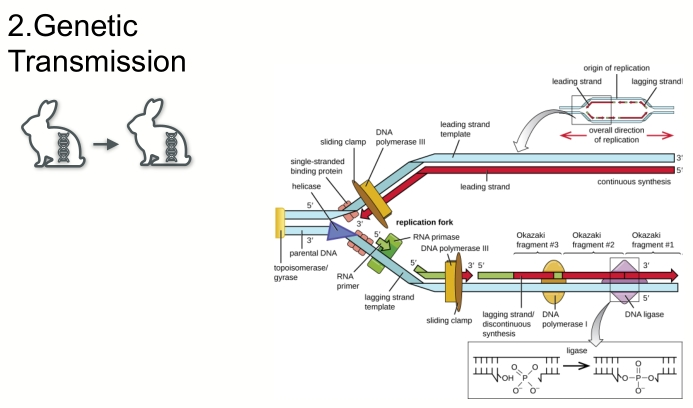
\includegraphics[width=0.9\textwidth]{DNA_replication_complex}
\end{figure}

\begin{figure}[H]
	\caption{Spontaneous formation and base pairing of plausible prebiotic nucleotides in water}\label{fig:SpontaneousFormation}
	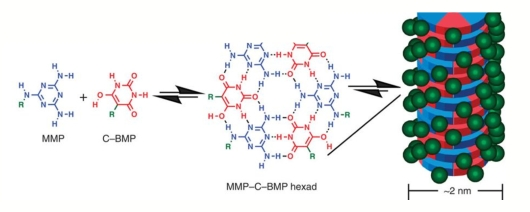
\includegraphics[width=0.9\textwidth]{SpontaneousFormation}
\end{figure}

\subsubsection{Evolution}

Genetic Transmission must ve sensitive enough to mutations for it to have an effect, but not too sensitive, so it doesn't break--Figure \ref{fig:EvolutionOfEvolution}.
\begin{figure}[H]
	\caption{DNA replication is complex and must be evolvable}\label{fig:EvolutionOfEvolution}
	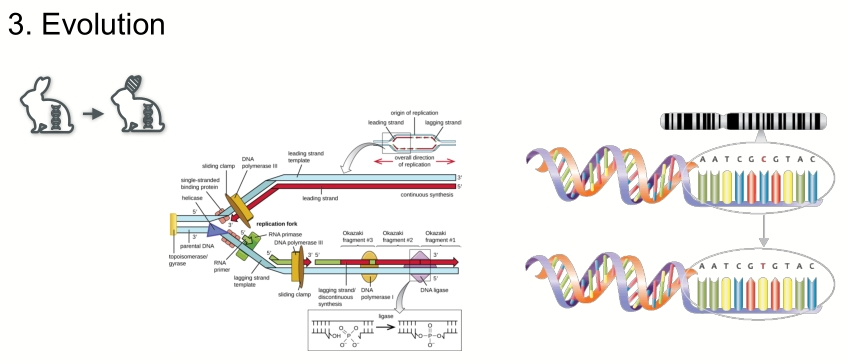
\includegraphics[width=0.9\textwidth]{EvolutionOfEvolution}
\end{figure}

We know that there were precursors to modern day heritable material probably around at the origin of life--Figure \ref{fig:SpontaneousFormation}\cite{cafferty2016spontaneous}. Could they change and still work? Yes: they mutate, and work in different ways--Figure \ref{fig:ContinuityInEvolution}\cite{fontana1998continuity}.

\begin{figure}[H]
	\caption{Continuity in Evolution: On the Nature of Transitions}\label{fig:ContinuityInEvolution}
	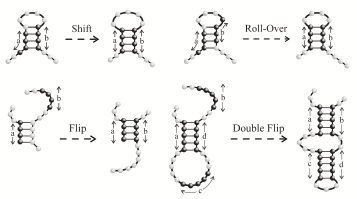
\includegraphics[width=0.9\textwidth]{ContinuityInEvolution}
\end{figure}
There are precursors for all the mechanisms we need. The big challenge is putting them together.
\begin{itemize}
	\item Preexisting Metabolism
	\item Simple Genetic Transmission
	\item Evolution in Simple Life
\end{itemize}

Suggested Reading
\begin{itemize}
	\item \cite{maynard1999origins} covers origins of life, eukaryotes, sex, society; 
	\item \cite{sumper1975evidence} treats life more mechanistically, and shows how we can use chemistry to understand it.
\end{itemize}

See also \cite{orgel2004prebiotic}, \cite{eigen1971selforganization}, \cite{kun2005real}, and \cite{ratcliff2014experimental}.

\subsection{A Recipe for Adaptation}

Lecturer: David Baum

Since the capacity for ]Adaptive Evolution is central to almost any definition of life, we need to understand what is the simplest system capable of undergoing adaptive evolution. Life is too complex to explain without an adaptive
process--Figure \ref{fig:LifeTooComplex}\cite{hoyle1983intelligent}. A cell is too complicated to  just emerge, so we need to think about how adaptation could start working on something simpler than a modern cell.

\begin{figure}[H]
	\caption{Life is too complex to explain without an adaptive
		process!}\label{fig:LifeTooComplex}
	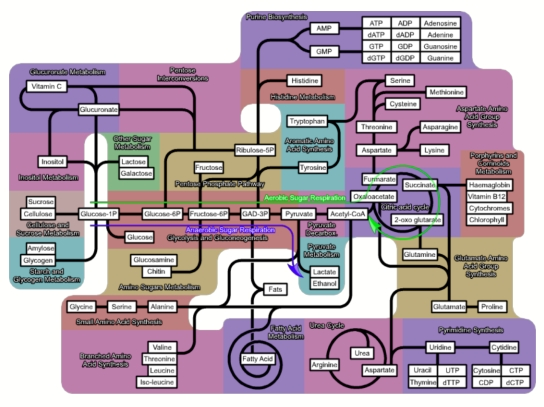
\includegraphics[width=0.9\textwidth]{LifeTooComplex}
\end{figure}

Figure \ref{fig:ReplicationMutationSelection} is a reminder of the way Darwinian Evolution works. Favoured variant \textit{could} be more complex. But, if you need cells and a genetic system to evolve adaptively it is hard to see how life can start--Figure \ref{fig:ChickenEgg}.
\begin{figure}[H]
	\caption{Darwinian evolution: Replication-Mutation- Selection}\label{fig:ReplicationMutationSelection}
	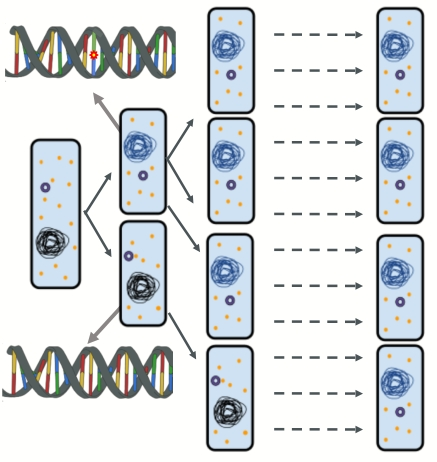
\includegraphics[width=0.9\textwidth]{ReplicationMutationSelection}
\end{figure}

\begin{figure}[H]
	\caption{if you need cells and a genetic system to evolve adaptively it is hard to see how life can start}\label{fig:ChickenEgg}
	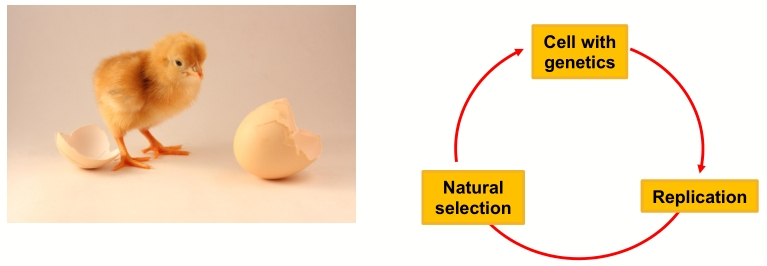
\includegraphics[width=0.9\textwidth]{ChickenEgg}
\end{figure}

There are a couple of ideas:

\begin{itemize}
	\item Cells could pass on their identity by passing on a
	dynamically maintained chemical state (analog)--Figure \ref{fig:CellWithoutGenes}.
	\item Self-replicating molecules could give rise to cells--Figure \ref{fig:GenesWithoutCells}.
\end{itemize}

\begin{figure}[H]
	\caption{Cells without genes}\label{fig:CellWithoutGenes}
	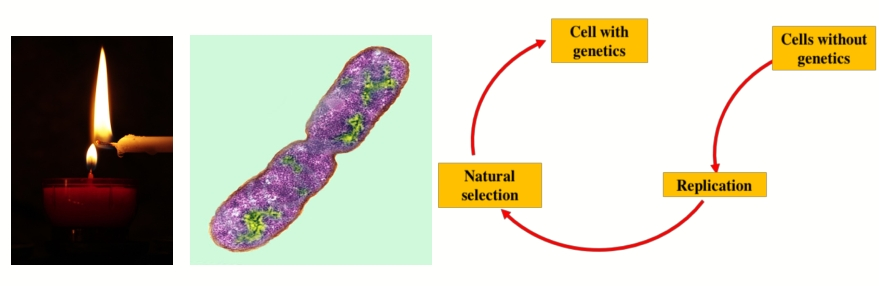
\includegraphics[width=0.9\textwidth]{CellWithoutGenes}
\end{figure}

\begin{figure}[H]
	\caption{Genes without cells}\label{fig:GenesWithoutCells}
	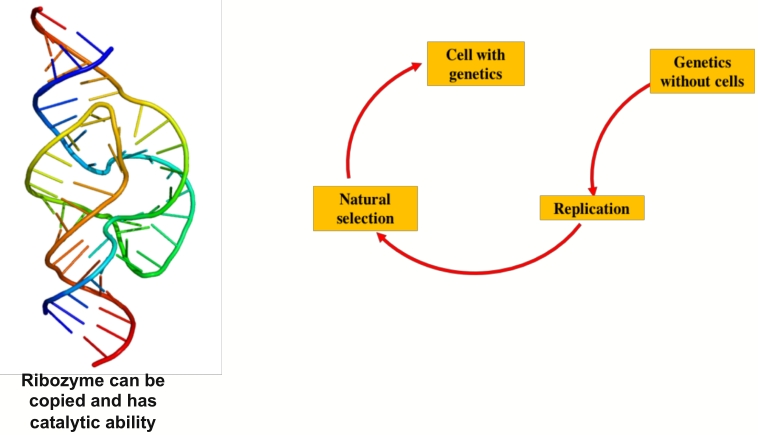
\includegraphics[width=0.9\textwidth]{GenesWithoutCells}
\end{figure}

Is this still too complex? Dividing protocells and self-replicating RNA could
be too complex to arise spontaneously. Nuclotides not likely to be sitting around in high abundance.

One possibility is no genetics and no cells. Adaptive material is possible if material in some sort of Spatial Structure--Figure \ref{fig:WangWang}\cite{wang2015evolution}.

\begin{figure}[H]
	\caption{Spatial structure does not require bounded cells}\label{fig:WangWang}
	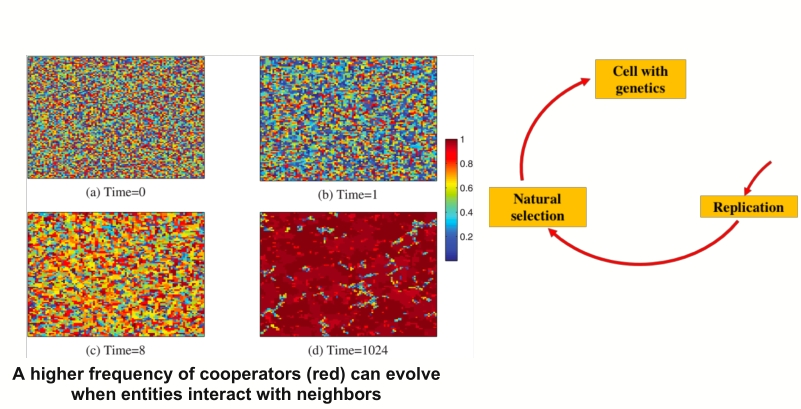
\includegraphics[width=0.9\textwidth]{WangWang}
\end{figure}

Perhaps the first adaptive evolving systems were flat living systems--Figure \ref{fig:Baum2018}\cite{baum2018origin}--slime-like things that lived on surfaces, had a metabolism, maintained a dynamics state, that could grow and evolve adaptively, and later give rise to cells. A cell can be seen as a very good way for a surface dweller to get to another surface--Figure \ref{fig:Baum2018}. One can imagine a situation in which, in an ancient ocean, there were minimal surfaces coated with life-like systems that could grow, spread, and be subjected to selection.

\begin{figure}[H]
	\caption{Spatial structure does not require bounded cells}\label{fig:Baum2018}
	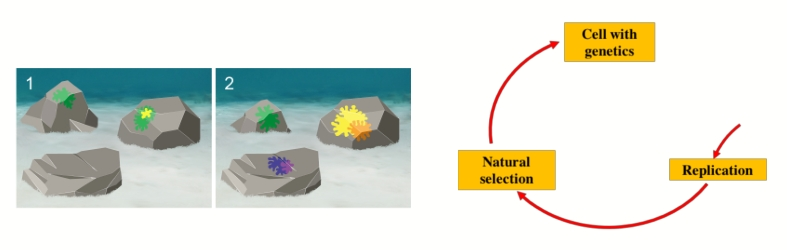
\includegraphics[width=0.9\textwidth]{Baum2018}
\end{figure}

Cells could have started as a transport mechanism--Figure \ref{fig:Baum2015}\cite{10.1093/biosci/biv063}--which enable certain types to spread.

\begin{figure}[H]
	\caption{Adaptive evolution started before cells or genetics}\label{fig:Baum2015}
	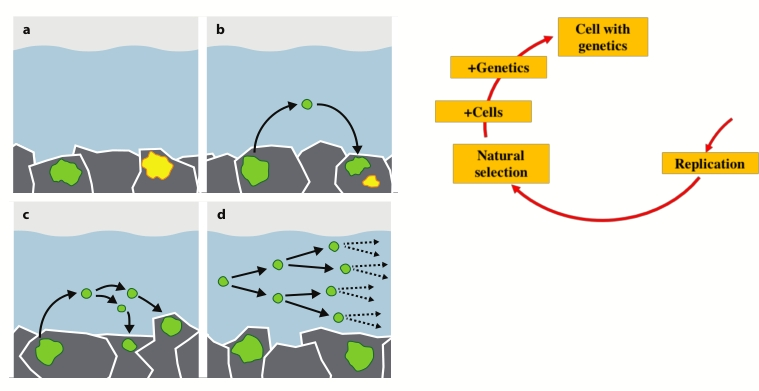
\includegraphics[width=0.9\textwidth]{Baum2015}
\end{figure}

To summarize, Evolutionary theory plays a central role--Figure \ref{fig:Baum2018a}\cite{baum2018origin}. It seems that cells with genetics are too complex, and we need a theory of simpler evolving progenitors.

\begin{figure}[H]
	\caption{Evolutionary theory plays a central role}\label{fig:Baum2018a}
	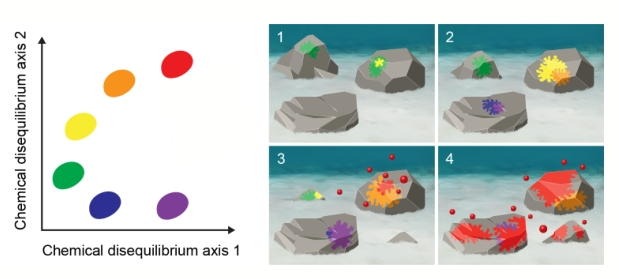
\includegraphics[width=0.9\textwidth]{Baum2018a}
\end{figure}


\subsection{Chance \& Change}

Lecturer: Andrew Rominger

Evolution is a theory of chance events, and change through time.

Evolution: Change in the heritable characteristics of
a \textit{population} through time--Figure \ref{fig:ChangeThroughTime}.
\begin{figure}[H]
	\caption{Evolution: Change in the heritable characteristics of
		a population through time}\label{fig:ChangeThroughTime}
	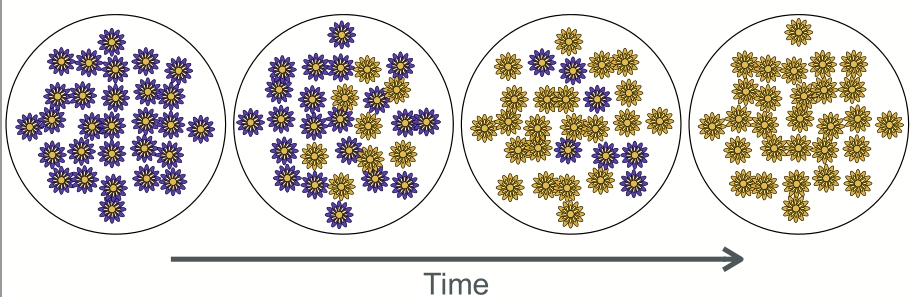
\includegraphics[width=0.9\textwidth]{ChangeThroughTime}
\end{figure}

Four key evolutionary processes
\begin{itemize}
	\item Reproduction (+ heritability)
	\begin{itemize}
		\item can ignore haploid/diploid if mating random
		\item maximum population size is finite
		\item Coalescence--Figure \ref{fig:Coalescence}
		\item Because Earth is finite and very old, LUCA is less an
		indication of the singularity of life’s origin and more a
		statistical artifact related to “Gambler’s ruin” 
	\end{itemize}
	\item Mutation
	\item Drift -- The fate of mutations without fitness consequences--Figure \ref{fig:Neutral} 
	\item Selection--The fate of mutations with fitness consequences--Figure \ref{fig:Selection}. Fitness is the differential reproductive
	success conferred by the new mutation.
\end{itemize}

\begin{figure}[H]
	\caption{Populations are finite $\implies$ Coalescence}\label{fig:Coalescence}
	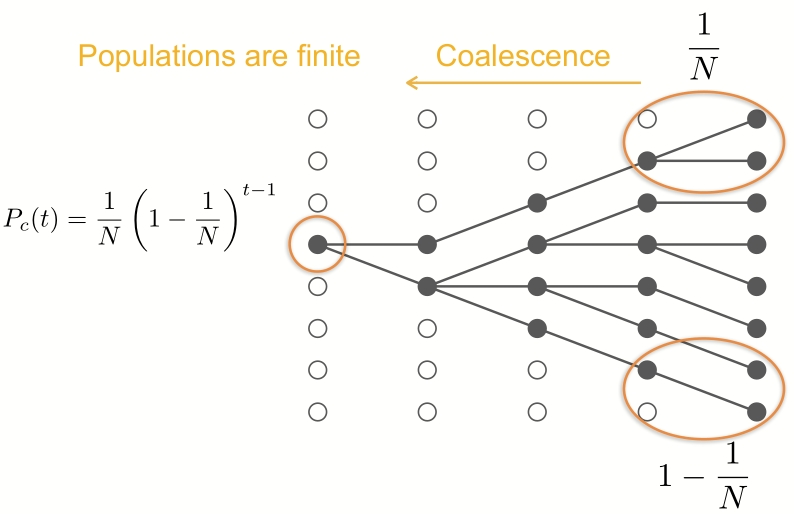
\includegraphics[width=0.9\textwidth]{Coalescence}
\end{figure}

\begin{figure}[H]
	\caption{The fate of mutations without fitness
		consequences}\label{fig:Neutral}
	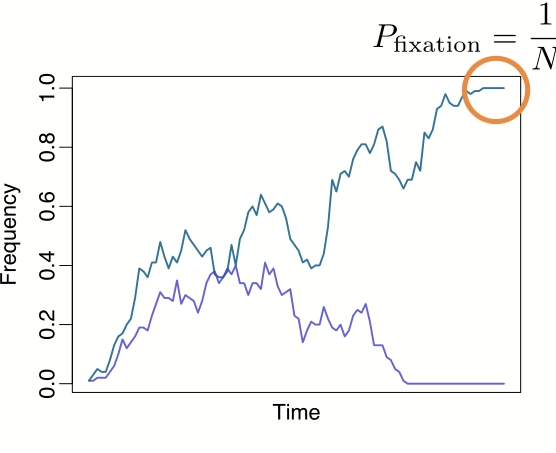
\includegraphics[width=0.9\textwidth]{Neutral}
\end{figure}

\begin{figure}[H]
	\caption{The fate of mutations with fitness
		consequences}\label{fig:Selection}
	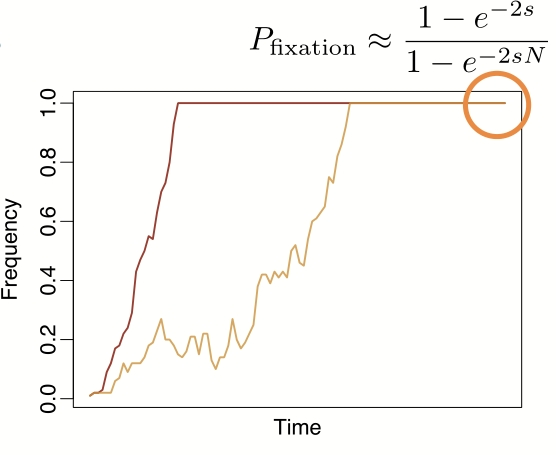
\includegraphics[width=0.9\textwidth]{Selection}
\end{figure}

Figure \ref{fig:MutationSpace} depicts \textit{Mutation Space}, a network of sequences connected by edges of single basepair mutations. Then we have a Fitness Landscape--Figure \ref{fig:FitnessLandscapeMovement}. Notice that probability of a mutation \textit{does not depend on fitness}, but fate does.
\begin{figure}[H]
	\caption{Mutations and sequence spaces}\label{fig:MutationSpace}
	\includegraphics[width=0.9\textwidth]{MutationSpace}
\end{figure}

\begin{figure}[H]
	\caption{Fitness landscapes}\label{fig:FitnessLandscapeMovement}
	\includegraphics[width=0.9\textwidth]{FitnessLandscapeMovement}
\end{figure}

NB: fitness isn't necessarily related to complexity! A priori any relationship is possible. So where does complexity come from? Maybe just a random walk?

Real World Complexities.

\begin{itemize}
	\item  Fluctuating population sizes
	\item  Non-random mating
	\item  Fluctuating environments and variable
	selection
\end{itemize}
\begin{figure}[H]
	\caption{Real World Complexities: how to cross a valley?}\label{fig:RealWorldComplexities}
	\includegraphics[width=0.9\textwidth]{RealWorldComplexities}
\end{figure}

Further reading: \cite{gillespie1984molecular}, \cite{kauffman1989nk}, \cite{kimura1983neutral}, \cite{kingman2000origins}, \cite{patwa2008fixation}, \cite{poelwijk2007empirical}, \cite{rosenberg2002genealogical}.

\section{Niche Construction}

% end of text 

% glossary
\printglossaries

% bibliography go here
 
\bibliographystyle{unsrt}
\addcontentsline{toc}{section}{Bibliography}
\bibliography{origins}

\end{document}
